\chapter{Introduction to Multimedia Data}
\label{chap:image}

\begin{abstract}{Abstract}
 
Digitally collected data often does not only contain texts, but also audio, images and videos. Instead of using only textual features as we did in previous chapters, we could as well use, for instance, pixel values
to analyse images. Without going into detail, in this chapter we will show how to store, represent and convert multimedia data in order to use it as an input in our computational analysis. We will discuss how to obtain text from images (OCR) and audio (speech-to-text), which allows to apply text analytics to  multimedia data. We will then focus on image analysis using machine learning classification techniques based on deep learning, and will explain how to build (or fine-tune) a Convolutional Neural Network (CNN) by ourselves, or to use a commercial service (Amazon Rekognition) to conduct this task. 
\end{abstract}

\keywords{Image, Audio, Video, Multimedia, Image Classification, Deep Learning}

\begin{objectives}
\item Learn how to transform multimedia data into useful inputs for computational analysis
\item Understand how to conduct deep learning to automatic classification of images
\end{objectives}

\begin{feature}
This chapter uses \pkg{PIL} (Python) and \pkg{imagemagic} (generic) to convert pictures as inputs; and \pkg{tesseract} (generic) and  Google 'Cloud Speech' API (\pkg{googleLanguageR} in and and \pkg{google\-cloud\-language} in Python) to convert into text images or audio files, respectively. We will use \pkg{Tensorflow} and \pkg{keras} (both in Python and R) to build and fine-tune CNNs.
\end{feature}

\section{Storing, representing, and converting images}
\label{sec:storing}

In this section we will focus on learning how to store, represent, and convert images for further computational analysis. You can also have a very nice and complete overview of computational analysis of images in \citet{williams2020images}.

To perform basic image manipulation we have to: (i) load images and transform their shape when it is necessary (by cropping or resizing), and (ii) to create a mathematical representation of the image (normally derived from it size, colors and pixel intensity) such of a 3D matrix or a flatten vector. You have some useful libraries in Python and R (\pkg{pil} and \pkg{imagemagik}, respectively) to conduct research in these initial stages, but you will also find that more advanced libraries in computer vision will include functions or modules for pre-processing images. At this point you can work either locally or remotely, but keep in mind that images can be heavy files and if you are working with thousands of files you will probably need to store or process them in the cloud (see Section~\ref{sec:cloudcomputing}).

You can load any image as an object onto your workspace as we show in \refex{load}. In this case we load and visualize two pictures of refugees published by mainstream media in Europe (see \citet{amores2019visual}), one is a JPG and the other is a PNG file. For this basic loading step we used the \fn{open} function of the \fn{Image} module in \pkg{pil} and \fn{image\_read} function in \pkg{imagemagik}. The JPG image file is a 805x453 picture with the color model \textit{RGB} and the PNG is a 1540x978 picture with the color model \textit{RGBA}. As you may notice the two objects have different formats, sizes and color models, which means that there is little analysis you can do if you don't create a standard mathematical representation of both. 

\pyrex[output=both,caption=Loading JPG and PNG pictures as objects]{chapter15/load}

\begin{figure}
\centering
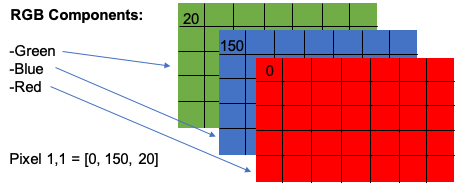
\includegraphics[width=0.9\linewidth]{figures/ch15_pixel.png}
\caption{Representation of the matrix data structure of a RGB image in which each pixel contains information for the intensity of each color component}
\label{fig:pixel}
\end{figure}

The good news when working with digital images is that the concept of \texttt{pixel} (picture element) will help you to understand the basic mathematical representation behind computational analysis of images. A rectangular grid of pixels is represented by a dot matrix which in turn generates a \texttt{bitmap image} or \texttt{raster graphic}. The dot matrix data structure is a basic but powerful representation of the images since we can conduct multiple simple and advanced operations with the matrices. Specifically, each dot in the matrix is a number that contains information about the intensity of each pixel (that commonly ranges from 0 to 255) also known as bit or color depth (figure~\ref{fig:pixel}). This means that the numerical representation of a pixel can have 256 different values being 0 the darkest tone of a given color and 255 the lightest. Keep in mind that if you divide the pixel values by 255 you will have a 0-1 scale to represent the intensity.

In a blank-and-white picture we will only have one color (grayscale), with the darker points representing the black and the lighter ones the white. The mathematical representation will be a single matrix or a two-dimensional array in which the number of rows and columns will correspond to the dimensions of the image. For instance in a 224 x 224 black-and-white picture we will have 50,176 integers (0-255 scales) representing each pixel intensity. 

In \refex{imagel} we convert our original JPG picture to grayscale and then create an object with the mathematical representation (a 453 x 805 matrix).

\pyrex[output=both,caption=Converting images to grayscale and creating a two-dimensional array]{chapter15/imagel}

By contrast, colour images will have multiple color channels that depend on the color model you chose. One standard color model is the  three-channel RGB (\textit{red}, \textit{green} and \textit{blue}), but you can find other variations in the chosen colors and the number of channels such as: RYB (\textit{red}, \textit{yellow} and \textit{blue}), RGBA (\textit{red}, \textit{green}, \textit{blue} and \textit{alpha}\footnote{Alpha refers to the opacity of each pixel} ) or CMYK (\textit{cyan}, \textit{magneta}, \textit{yellow} and \textit{key}\footnote{Key refers to \textit{black}}).  We will mostly use RGB in this book since it is the most used representation in the state-of-the-art literature in computer vision given that these color channels yield more accurate models. RGB's mathematical representation will be a three-dimensional matrix or a collection of three two-dimensional arrays (one for each color). Then a RGB 224 x 224 picture will have 50,176 pixel intensities for each of the three colors, or in other words a total of 150,528 integers!

Now, in \refex{imagergb} we convert our original JPG file to a RGB object and then create a new object with the mathematical representation (a 453 x 805 x 3 matrix).

\pyrex[output=both,caption=Converting images to RGB color model and creating three two-dimensional arrays]{chapter15/imagergb}

Instead of pixels, there are other ways to store digital images. One of them is the \textit{vector graphics}, with formats such as .ai, .eps, .svg or .drw. Differently to bitmap images, they don't have a grid of dots but a set of \textit{paths} (lines, triangles, square, curvy shapes, etc.) that have a start and end point, so simple and complex images are created with paths. The great advantage of this format is that images do not get "pixeled" when you enlarge them because the paths can easily be transformed 	while remaining smooth. However, to obtain the standard mathematical representation of images you can easily convert (back and forth) the vector graphics to raster graphics such as RGB.

Sometimes you need to convert your image to a specific size. For example, in the case of image classification this is a very important step since all the input images of the model must have the same size. For this reason, one of the most common tasks in the preprocessing stage is to change the dimensions of the image in order to adjust width and height to a different size. In \refex{resize} we use \fn{resize} function in \pkg{pil} and \fn{image\_scale} function in \pkg{imagemagik} to reduce the first of our original pictures in RGB (\texttt{my\_image1\_RGB}) to 25\% . Notice that we first obtain the original dimensions of the photograph (i.e. \texttt{my\_image1\_RGB.width} or \verb|image_info(my\_image1\_RGB)['width'][[1]]|) and then multiply by 0.25 in order to obtain the new size which is the argument required by the functions.

\pyrex[output=both,format=png,caption=Resize to 25\% and visualize a picture]{chapter15/resize}

Now, using the same functions of the latter example, we specify in \refex{resize2} how to resize the same picture to 224 x 244, which is one of the standard dimensions in computer vision. 

\pyrex[output=both,format=png,caption=Resize to 224 x 224 and visualize a picture]{chapter15/resize2}

You may have noticed that the new image has now the correct width and height but that it looks deformed. The reason is that the original picture was not squared and our order was to forcedly fit it into a 224 x 224 square, loosing its original aspect. There are different alternative to solve this issue, but probably the most extended is to \textit{crop} the original image to create a squared picture. As you can see in \refex{crop} we can create a function that first determines the orientation of the picture (vertical versus horizontal) and then cut the margins (upper and down if it is vertical; and left and right if it is vertical) to create a square. After applying this ad hoc function \fn{crop} to the original image we can resize again to obtain a non-distorted 224 x 224 image.

Of course you are loosing now part of the picture information, so you may think of other alternatives such as filling a couple of sides with blank pixels (or \texttt{padding}) in order to create the square by adding information instead of removing.

\pyrex[output=both,format=png,caption=Function to crop the image to create a square and the resize the picture]{chapter15/crop}

You can also adjust the orientation of the image, flip or flop it, or change its background, among other commands. These techniques might be useful for creating extra images in order to enlarge the training set in image classification (see xxx). This is called \textit{data augmentation} and consists for duplicating the initial examples from where the model learn and give them some twist so the algorithm can be more robust and generalize better. In \refex{crop} we used the \fn{rotate} method in \pkg{pil} and \fn{image\_rotate} function in \pkg{imagemagik} to rotate 45 degrees the above resized image \texttt{my\_image1\_RGB\_224} to see how easy we can get an alternative picture with similar information to include in an augmented training set.

\pyrex[output=both,format=png,caption=Rotating 45 degrees a picture]{chapter15/rotate}

Finally, the numerical representation of visual contents can help us to \textit{compare} pictures in order find similar or even duplicate images. Let's take the case of RGB images which in \refex{imagergb} we showed how to transform into a three two-dimensional array. If we now convert the 3D matrix of the image into a flatten vector we can use use new simpler numerical representation to estimate similarities. Specifically, as we do in \refex{flatten}, we can take the vectors two \textit{flatten images} of resized 15 x 15 images to ease computation (\texttt{img\_vect1} and \texttt{img\_vect2}) and use \textit{cosine similarity} to estimate how akin those images are. We stacked the two vectors in a matrix and then used the \fn{cosine\_similarity} function of the \fn{metrics} module of the  \pkg{sklearn} package in Python and \fn{cosine} function of the \pkg{lsa} package in R.

\pyrex[output=both,caption=Comparing two flatten vectors to detect similarities between images]{chapter15/flatten}
 
As you can notice in the resulting matrix when the images are compared with themselves (that would be the case of an exact duplicate) the obtain a value of 1. Similar images would obtain values under 1 but still close to it, while dissimilar images would obtain low values.

\section{Optical character recognition and speech-to-text}
\label{sec:ocr}

How to convert scanned documents into text files for further analysis. 
\section{Image classification}
\label{sec:cnn}

In this section, we will learn how to conduct computational image classification which is probably the most extended supervised machine learning application in the field of automatic analysis of images in communication and social sciences. We will firstly discuss how to apply a \textit{shallow} algorithm and then a deep-learning approach, given a labelled data set. 	

In an image classification task we train a model with examples (e.g. a corpus of pictures with labels) in order to predict the category of any given new sample. It is the same logic used in supervised text classification  explained in Section~\ref{sec:supervised} but suing images instead of texts. For example, if we show many pictures of cats and many of houses the algorithm would learn the constant features in each and will tell you with some degree of confidence if a new picture contains either a cat or a house. It is the same with letters, numbers, objects or faces, and you can apply either binary or multi-class classification. Just think when your vehicle registration plate is recognized by a camera or when your face is automatically labelled in pictures posted in Facebook.

Beyond image classification we have other specific tasks in computer vision such as \textit{object detection} or \textit{semantic segmentation}. To conduct object detection we have first to locate all the possible objects contained in a picture by predicting a bounding box (i.e. height and weight, as well as the four points corresponding to the vertical and horizontal coordinates of the center of the object), which is normally an regression task. Once the bounding boxes are placed around the objects, we must apply multi-class classification as explained earlier. In the case of semantic segmentation, instead of classifying objects, we classify each pixel of the image according to the class of the object the pixel belong to, which means that different objects of the same class might not be distinguished. Figure~\ref{fig:location} shows an example of each of these techniques presented by \citet{geron2019hands}.

\begin{figure}
\centering
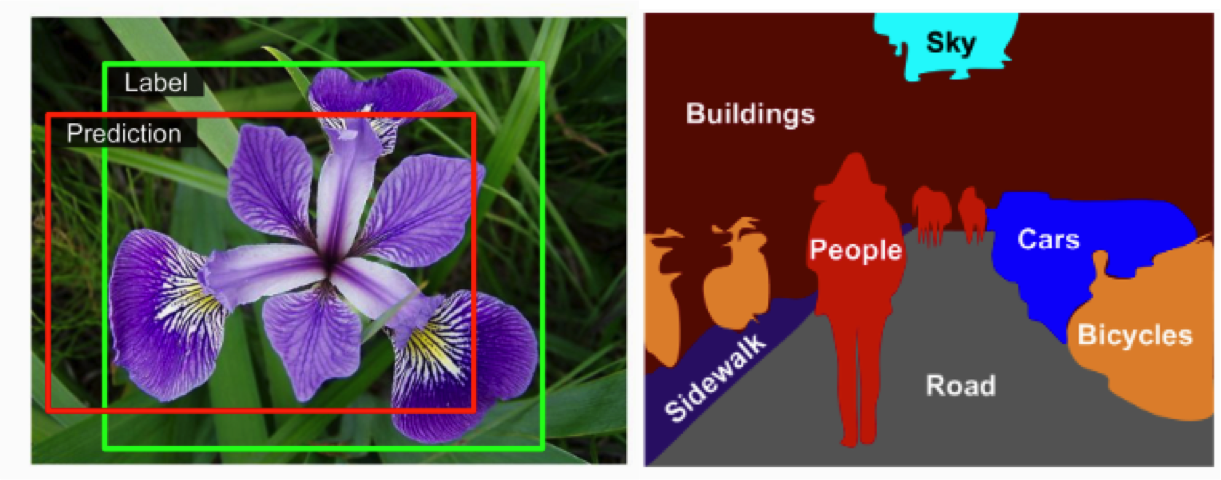
\includegraphics[width=0.9\linewidth]{figures/ch15_location.png}
\caption{Object detection (left) versus semantic segmentation (right).
Source: \citet{geron2019hands}}
\label{fig:location}
\end{figure}

It is beyond of the scope of this book to address the implementation of object detection or semantic segmentation, but we will focus on how to conduct basic image classification in state-of-the-art libraries in R and Python. As you may have imagined we will need some already-labelled images to have a proper training set. It is also out of the reach of this chapter to collect and annotate the images, which is the reason why we will mostly rely on pre-existing image databases (i.e. MINST or Fashion MINST) and pre-trained models (i.e. CNNs architectures), or will provide you with ad hoc annotated images if it is necessary. 

\subsection{Basic classification with shallow algorithms}
\label{subsec:shallow}

In Chapter~\ref{chap:introsml} we introduced you into the exciting world of machine learning and in Section~\ref{sec:supervised} we showed how to used the \textit{supervised} approach to classify texts. Most of the discussed models were based in the so called \textit{shallow} algorithms (Naïve Bayes, Regression, Support Vector Machines, Decision Trees or Random Forest), in opposition to other algorithms liked to \textit{deep} learning. As we will see in the next section, deep neural networks are nowadays the best option for complex tasks in image classification. However, we will now explain how to conduct simple multi-class classification of images that contain numbers with some shallow algorithms.

Let us begin by training a model to recognize numbers using 70,000 small images of digits handwritten from the Modified National Institute of Standards and Technology (MNIST) dataset. This popular training corpus contains gray-scale examples of numbers written by American students and workers and it is usually employed to test machine learning models (60,000 for training and 10,000 for testing). Image sizes are 28 x 28, which generates 784 features for each image, with pixels values from white to black represented by a 0-255 scales. In Figure~\ref{fig:numbers} you can observe the 

\begin{figure}
\centering
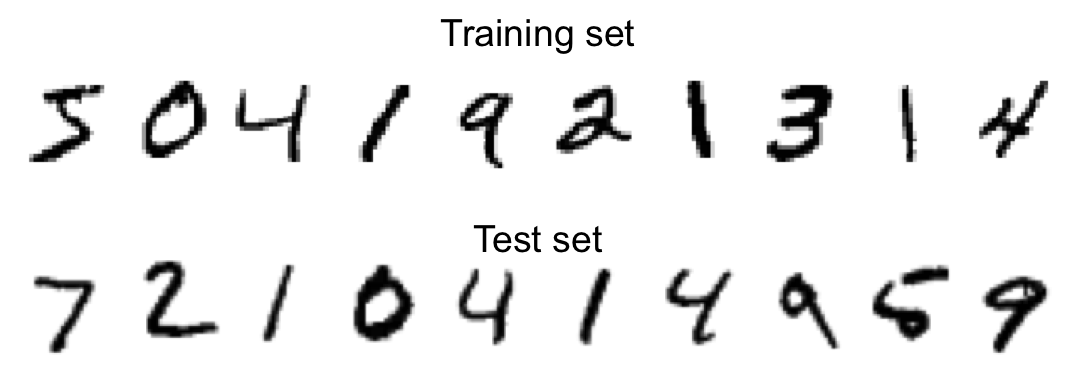
\includegraphics[width=0.9\linewidth]{figures/ch15_numbers.png}
\caption{First 10 handwritten digits from the training and test set of the MNIST}
\label{fig:numbers}
\end{figure}

In \refex{mnist} we...

\pyrex[output=both,caption=XXX]{chapter15/mnist}

And in \refex{multiclass}  we    with 100 trees ... obtain an accuracy over 0.97

\pyrex[output=both,caption=XXX]{chapter15/multiclass}



\subsection{Deep learning for image analysis}
\label{subsec:deep}

MLP for image classification p 297   Fashion MNIST (https://github.com/zalandoresearch/fashion-mnist)

\subsection{Fine tuning an open source CNN}
\label{subsec:deep}

Fine tuning an open source CNN   RestNet 18? (Andreu example)
\section{Using existing libraries and APIs}
\label{sec:apivisions}

In the next sections we will show you how to deal with multimedia contents from scratch, with special attention to image classification using state-of-the-art libraries. However, it might be a good idea to begin by using some existing libraries that directly implements multimedia analysis or by connecting to commercial services to deploy classification tasks remotely using their APIs. There is a vast variety of available libraries and APIs, which we cannot cover in this book, but we will briefly mention some of them that may be useful in the computational analysis of communication.

One example in the field of visual analytics is the \textit{optical character recognition} (OCR). It is true that you can train your own models to deploy multi-class classification and predict every letter, number or symbol in an image, but it will be a task that will take you a lot of effort. Instead, there are specialized libraries in both R and Python such as \pkg{tesseract} that deploy this task in seconds with high accuracy. It is still possible that you will have apply some pre-processing to the input images in order to put them on shape. This means that you may need to use packages such as \pkg{PIL} or \pkg{Magick} to improve the quality of the image by cropping it or by reducing the background noise.  In the case of PDFs files you will have to convert them first into images and then apply OCR.

In the case of more complex audio and image documents you can use more sophisticated services provided by private companies (i.e. Google, Amazon, Microsoft, etc.). These commercial services have already deployed their own machine learning models with very good results. Some times you can even customize some of their models, but as a rule their internal features and configuration are not transparent to the user. Moreover, these services offer friendly APIs and normally a free quota to deploy your first exercises.

To work with audio files, many social researchers might need to convert long conversations, radio programs, or interviews to plain text. For this propose, \textit{Google Cloud} offer the service \textit{Speech-to-Text}\footnote{https://cloud.google.com/speech-to-text}  that remotely transcribe the audio to a text format supporting multiple languages (more than 125!). With this service you can remotely use the advanced deep learning models created by Google Platform from your own local computer (you must have an account and connect with the proper packages such as \pkg{googleLanguageR} or \pkg{google-cloud-language} in Python).

If you apply either OCR to images or Speech-to-Text recognition to audio contents you will have juicy plain text to conduct NLP, sentiment analysis, topic modelling, among other techniques.  Thus, it is very likely that you will have to combine different libraries and services to perform a complete computational pipeline, even jumping from R to Python, and vice versa!

Finally, we would like to mention the existence of commercial services of \textit{autotaggers}, such as Google's Cloud Vision, Microsoft's Computer Vision or Amazon's Recognition. For example, if you connect to the services of Amazon's Recognition you can not only detect and classify images, but also conduct sentiment analysis over faces or predict sensitive contents within the images. As in the case of Google Could, you will have to obtain commercially sold credentials to be able to connect to Amazon's Recognition API (also with a free initial quota). This approach has two main advantages. The first is the access to a very well trained and validated model (continuously re-trained) over millions of images and with the participation of thousands of coders. The second is the scalability because you can store and analyze images at scale at a very good speed using cloud computing services.

\begin{figure}
\centering
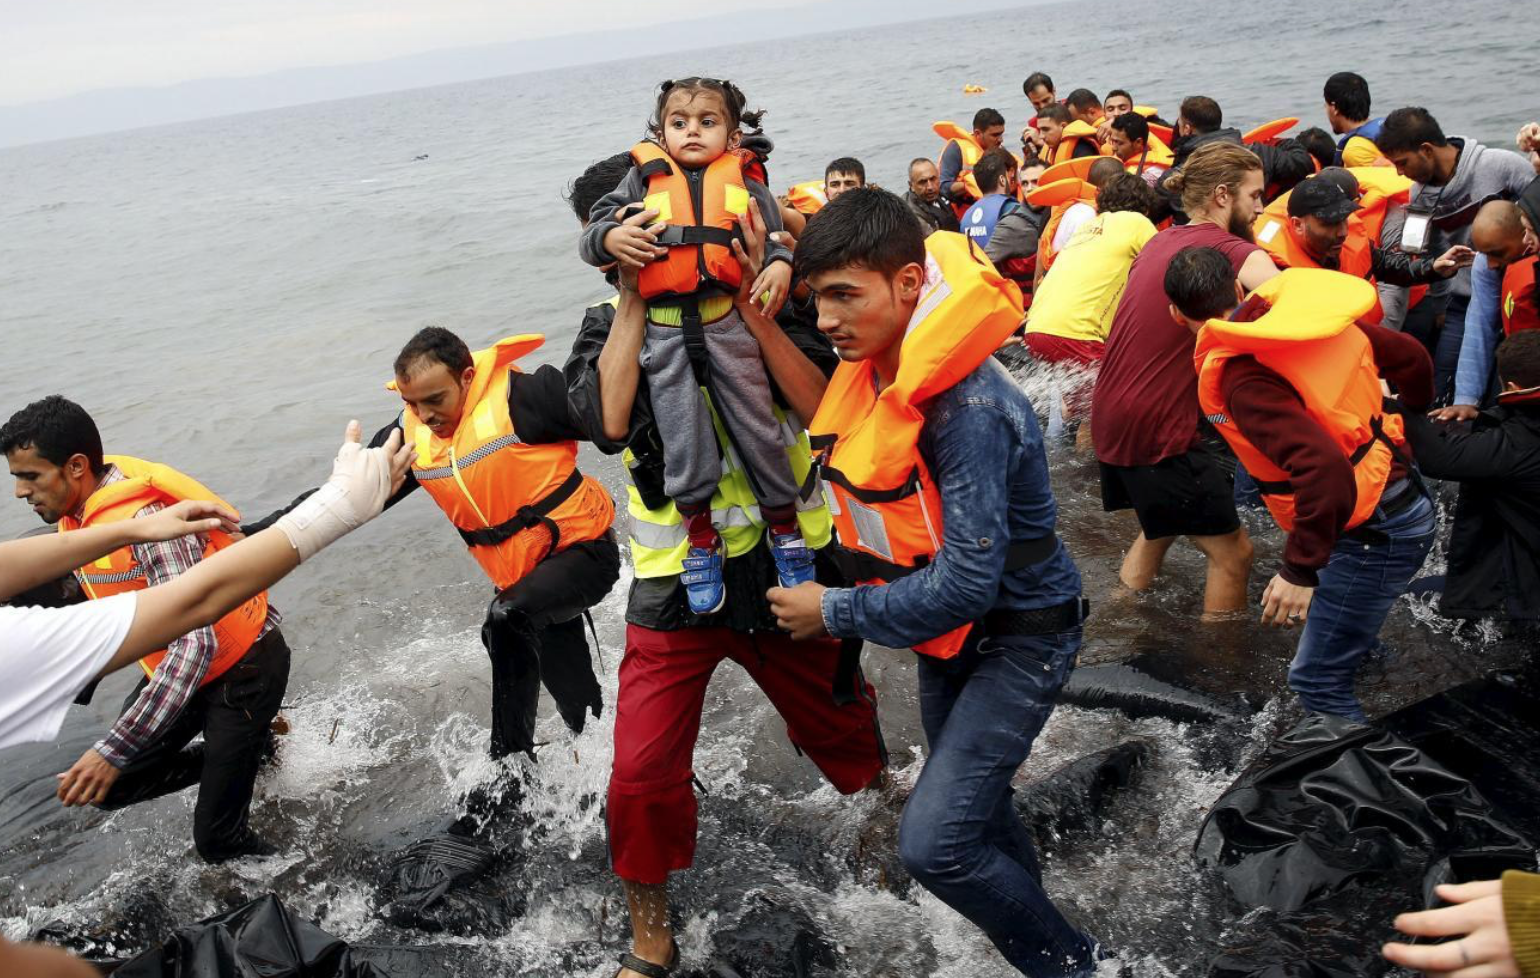
\includegraphics[width=0.9\linewidth]{figures/ch15_refugees.png}
\caption{By using Amazon's Recognition API
A photograph of refugees on a lifeboat, used as an input for Amazon's Recognition API. The commercial service detects in the pictures classes such as clothing\, apparel\, human\, person\, life jacket or vest.}
\label{fig:refugees}
\end{figure}

As an example, you can use Amazon's Recognition to detect objects in a news photograph of refugees in a lifeboat (Figure~\ref{fig:refugees}) and you will obtain a set of accurate labels: \textit{Clothing} (99.95\%), \textit{Apparel} (99.95\%), \textit{Human} (99.70\%), \textit{Person} (99.70\%), \textit{Life jacket} (99.43\%) and \textit{Vest} (99.43\%). With a lower confidence you will also find labels such as \textit{Coat} (67.39\%) and \textit{People} (66.78\%). This example also highlights the need for validation, and the difficulty of grasping complex concepts in automated analyses: While all of these labels are arguably correct, it is safe to say that they fail to actually grasp the essence of the picture and the social context. One may even go as far as saying that -- knowing the picture is about refugees -- some of these labels, were they given by a human to describe the picture, would sound pretty cynical.

In Section~\ref{sec:cnn} we will use this very same image (stored as \texttt{my\_image2\_RGB}) to detect objects using a classification model trained with an open-access database of images (ImageNet). You will find that there are some different predictions in both methods, but especially that the time to conduct the classification is shorter in the commercial service, since we don't have to train or choose a model. As you may imagine, you cannot neither modify the commercial models nor have access to their internal details, which is a strong limitation if you want to build your own and customized classification system.
